\chapter{Programming - Block Program}
\section{Overview}\paragraph*{The}\textbf{Programming - Block Program} screen (Figure 8.1) provides the Operator programming access to the \textbf{Block Program Details} used while in \textit{Auto} mode. The Operator is able to create and edit block programs. Navigation is possible to the main \textbf{Alarm} screen, the \textbf{Saw Parameters} screen, the \textbf{Check Program} screen,the \textbf{Vertical Axis} and \textbf{Cross Travel Axis} and \textbf{Long Travel Axis} manual screens, and of course the \textbf{Main} operation screen.
\begin{figure}
	\centering
	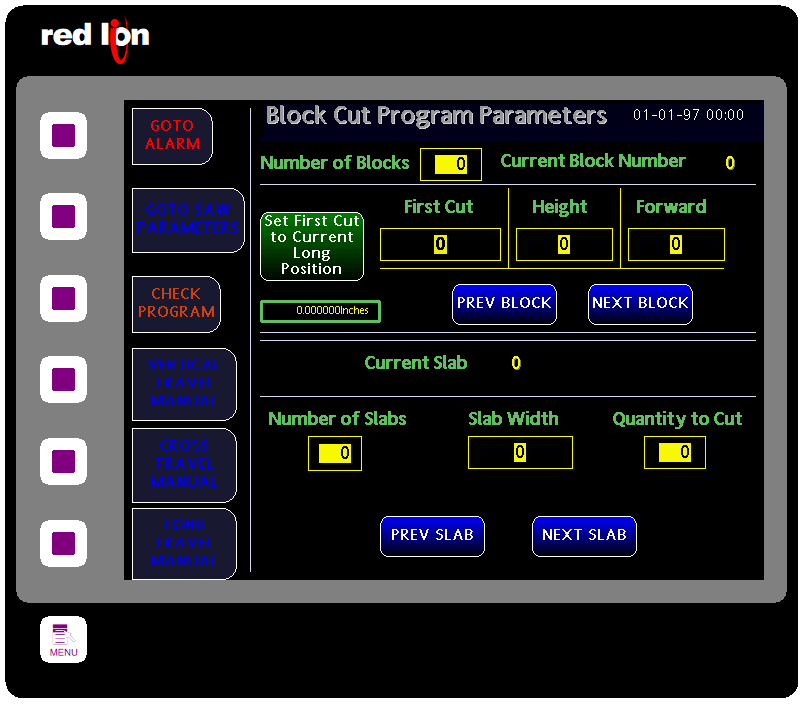
\includegraphics[width=0.5\linewidth]{screen-captures/program/cut-pgm}
	\caption{Programming - Block Program}
	\label{fig:prg-block-det}
\end{figure}
\section{Details}\paragraph*{The}\textbf{Block Program} screen details are divided into the following categories ...
\begin{list}{$\diamond$}{}
	\item \textbf{Screen Navigation}
	\item \textbf{Block Details}
	\item \textbf{Slab Details}
\end{list}
\pagebreak
\subsection{Screen Navigation}
\paragraph*{Is}performed by using the programmable Function Keys (FKeys) located down the left hand side of the OI Terminal (refer to Figure 5.2). The Operator may navigate to the following screens ...
\begin{list}{$\diamond$}{}
	\item \textbf{GOTO ALARM} Navigate to Alarm Screen.
	\item \textbf{GOTO SAW PARAMETERS} Navigate to Saw Parameter Screen.
	\item \textbf{CHECK PROGRAM} Navigate to Block Program Check Screen.
	\item \textbf{VERTICAL MANUAL} Navigate to Vertical Manual Control Screen.
	\item \textbf{CROSS TRAVEL MANUAL} Navigate to Cross Travel Manual Control Screen.
	\item \textbf{LONG AXIS MANUAL} Navigate to the Long Axis Manual Control Screen.
\end{list}
\begin{figure}
	\centering
	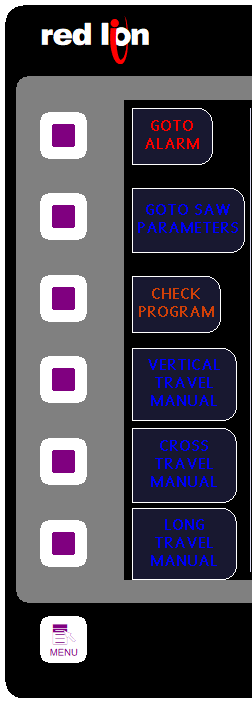
\includegraphics[width=0.2\linewidth]{screen-captures/program/cut-pgm-nav}
	\caption{Block Program Screen Navigation}
	\label{fig:cut-pgm-screen-nav}
\end{figure}
\paragraph{\textbf{\LARGE \textcolor{blue}{i}}}
The Menu Key located on the terminal at the lower left below the FKey's, will return the Operator to the Main Screen, from all other screens.\\
\begin{minipage}{4cm}
	\begin{picture}(20,70)
		
\includegraphics[width=.5\linewidth]{screen-captures/menu}
	\end{picture}
\end{minipage}\begin{minipage}[]{11cm}
	\paragraph{\textbf{\LARGE \textcolor{blue}{i}}} The Menu Key is pictured as it looks on the Terminal.
\end{minipage}
\pagebreak
\subsection{Block Details}\paragraph*{Blocks}are the actual stone blocks as laid out on the cutting floor by the Operator. The details about the block that are used in the program are shown in Figure 8.3. The \textbf{\textit{Number of Blocks}} is set by the Operator according to the actual block count on the cutting bed. The \textbf{\textit{Current Block Number}} indicates to the Operator which block they are actively programming, it is not settable. The PushButton \textbf{\textit{Set First Cut to Current Long Position}} will set the First Cut for the active block to the actual Long Axis Position (displayed below the button). Of course, the Operator could just enter a desired \textbf{\textit{First Cut}} in the entry field provided. The \textbf{\textit{Block Height}} must be entered by the Operator, this determines where the depth of the first cut for the block ends up as a result of the equation \textit{Block Height - Cut Depth}. The \textbf{\textit{Forward Position}} for Cross Travel is entered by the Operator, to tell the saw when the blade is out of rock. Since the Cross Travel will drift a fair amount when stopping, this should be treated as the minimum distance desired to ensure the blade has left the rock safely. The \textbf{\textit{PREV BLOCK}}
 and \textbf{\textit{NEXT BLOCK}} buttons are used to scroll through the blocks to be programmed. They are only active if there is a next or previous block to view. If a block is desired to be cut with only a \textit{First Cut} and no slabs, then the Operator would need to ensure that there is a zero (0) in the \textbf{\textit{Number of Slabs}} entry field of the Slab Details (Section 8.2.3).
	\paragraph{}
		\begin{figure}
			\centering
			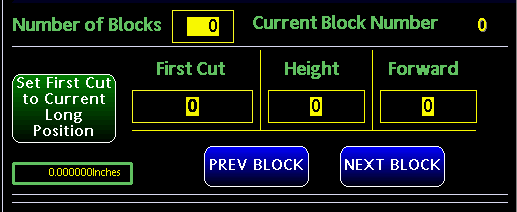
\includegraphics[width=.2\linewidth]{screen-captures/program/cut-pgm-block}
			\caption{Block Details Entry Fields}
			\label{fig:cut-pgm-block-entry}
		\end{figure}
	\paragraph{\textbf{\LARGE \textcolor{blue}{i}}}The Operator should use the Check Program pages to review the \textit{Block Program} that was entered in a table form which shows details about each block and slab. Also, it is strongly advised to reset both the block program and the automatic sequence before entering a new block program. This can be done on the first \textbf{\textit{CHECK PROGRAM}} screen.
\paragraph*{\textbf{{\LARGE \textcolor{red}{!}}}}A fault will be triggered by the program logic if the Operator tries to begin an Automatic Cycle without first entering a valid cut program. The Block Height is a critical dimension, if not correct, it can result in damage to the saw blade.
\pagebreak
\subsection{Slab Details}\paragraph*{Slabs}are the actual slabs to cut from the blocks as laid out on the cutting floor by the Operator. The details about the slabs that are used in the program are shown in Figure 8.4. The \textbf{\textit{Number of Slabs}} is set by the Operator according to the actual slab count of different sizes that are being cut from the active block. The \textbf{\textit{Cut Width}} entry field is where the Operator sets the width of the slab or slab size. The \textbf{\textit{Quantity to Cut}} is where the Operator enters the number of slabs of that particular size to cut from the selected block. The \textbf{\textit{PREV SLAB}}
and \textbf{\textit{NEXT SLAB}} buttons are used to scroll through the slabs to be programmed for the active block. They are only active if there is a next or previous slab to view.
\begin{figure}
	\centering
	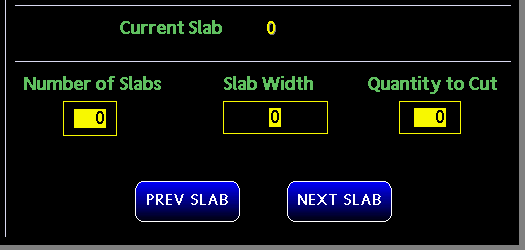
\includegraphics[width=.2\linewidth]{screen-captures/program/cut-pgm-slab}
	\caption{Slab Details Entry Fields}
	\label{fig:cut-pgm-slab-entry}
\end{figure}
\paragraph{\textbf{\LARGE \textcolor{blue}{i}}}The Operator should use the Check Program pages to review the \textit{Block Program} that was entered in a table form which shows details about each block and slab. Also, it is strongly advised to \textbf{reset} both the block program and the automatic sequence \textbf{before} entering a new block program. This can be done on the first \textbf{\textit{CHECK PROGRAM}} screen.